\subsubsection{Pseudemys --- Cooters and Redbellies}
\begin{center}
\begin{longtabu} to \textwidth {| | p{3.5cm} | X | |}

	\hline
	Taxonomy/Ancestry &
	subfamily Deirochelyinae. 7 species, validity of some taxa in question. referred to as cooters from kuta, word for turtle in Bambara and Malinke languages.
	
	\begin{center} 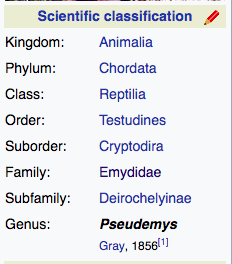
\includegraphics[scale=0.5]{testudines/emydidae/pseudemys/tax} \end{center}
	 \\
	\hline
	Size & 
	among the largest of the Emydids, they have carapace lengths reaching 17.3 in (44 cm) and weigh up to 22 lb (10 kg).
	\\
	\hline
	Color &
	black head w/ light lines running toward snout.
	 \\
	\hline
	Anatomy &
	they have a dark, highly domed carapace w/ large webbed feet to navigate strong currents.
	
	the hatchling has a round carapace, 1.5 in (4 cm) in diameter, green w/ bright yellow markings.
	 \\
	\hline
	Dimorphism & 
	females larger than males.
	\\
	\hline
	Behavior & 
	\begin{itemize}[noitemsep]
		\item bask on logs/sun-warmed rocks, often w/ other aquatic basking turtles (e.g. sliders, painteds)
		\item diurnal, wake w/ morning sun to bask/forage
		\item wander b/w bodies of freshwater $\rightarrow$ develop relatively large home range
		\item sleep under water vegetation
		\item cooler climate cooters = dormant during winter up to 2 months in underwater mud. do not breathe but take in oxygen from water thru cloaca
	\end{itemize}
	\\
	\hline
	Habitat & 
	usually found found in rivers w/ moderate current, lakes, or tidal marshes w/ heavy vegetation. they collect on the peninsular floodplains. they care capable of tolerating freshwater and brackish water.
	\\
	\hline
	Distribution & 
	native to central/eastern US, from Virgina south to mid-Georgia, west to eastern Texas, Oklahoma, north to southern Indiana. some populations in Rio Grande, Mexico.
	\\
	\hline
	Feeding Ecology & 
	\begin{itemize}[noitemsep]
		\item highly omnivorous, they will eat plants or animals, dead or alive
		\item they cannot swallow out of water, so they will leave to chase a prey item and then return to swallow it
		\item they chase, kill, and eat small fish
		\item they find carrion along the river edge
		\item tooth-like cusps in upper jaw function as an adaptation to aid in eating leaves/fibrous vegetation
		\item primarily, they consume a wide variety of aquatic plants, some terrestrial near water edge
		\item can take calcium thru separate source (e.g. cuttlebone) to self-regulate intake
		\item young tend to seek more protein-enriched (meat) diet
		\item hatchings predated upon by avian/mammal predators: skunks/raccoons, bull frogs, herons, snapping turtles, predatory fish, alligators, muskrats
	\end{itemize}
	\\
	\hline
	Reproductive Biology & 
	similar to the red-eared slider, they mate in early spring. as part of courtship, the male uses claws to flutter at the female's face and sniffs the female's tail for a pheromone signal. he swims above the female, stroking her face. if she is receptive, she will sink to the bottom of the river and allow the male to mount.
	
	after several weeks, the female crawls to land seeking a nesting site in May-June. she typically chooses sandy/loamy soil in an open area, within 100 ft (300 m) of the water's edge. she lays 10-25 eggs in 1 or more clutches, yielding ellipsoidal, 1.5 in (4 cm) long eggs. incubation time is determined by the temperature and ranges from 90-100 days. 
	
	eggs hatch within 45-56 days in August-September. they usually remain in the nest through the 1st winter. nearly 100\% of offspring will die the 1st year.
	\\
	\hline
	Ecological Role &
	
	\\
	\hline
	Conservation Status & 
	Threatened by loss of habitat, predation, highway death, use as food source, pet industry, but hardy as a whole, continues to thrive. LC.
	\\
	\hline
\end{longtabu}
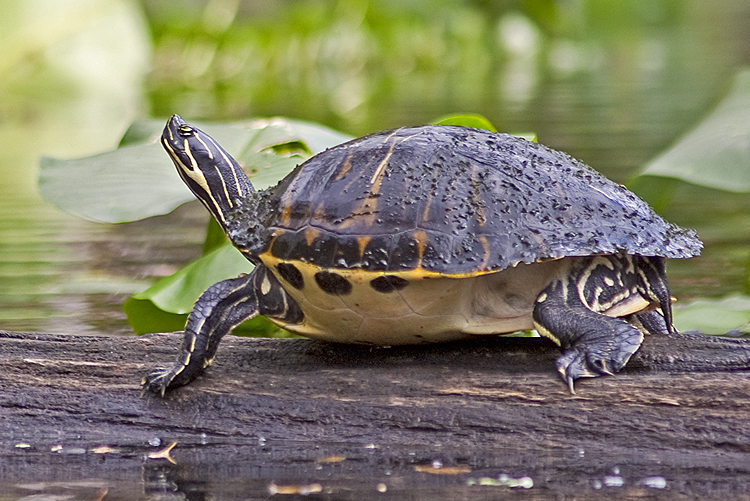
\includegraphics[scale=0.85]{testudines/emydidae/pseudemys/1}
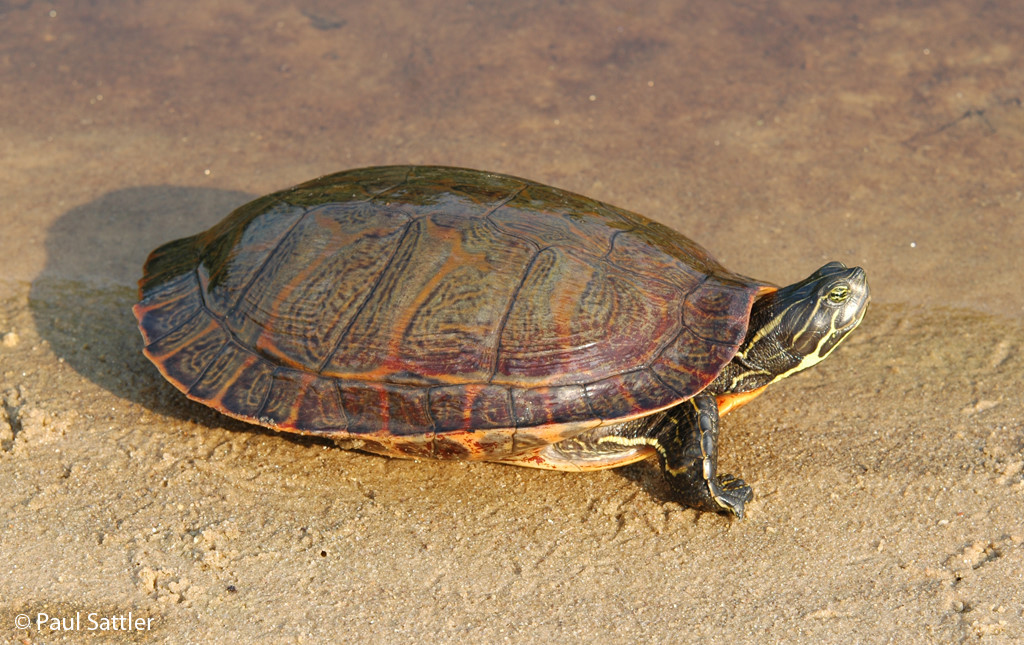
\includegraphics[scale=0.85]{testudines/emydidae/pseudemys/2}
\end{center}